\begin{exercise}
    \item 下列哪组矢量是一组基底?
    \begin{enumerate}
        \item $\bb{g}_1\sim (4,6,2),\bb{g}_2\sim (1,0,1),\bb{g}_3\sim (1,3,0)$
        \item $\bb{g}_1\sim (1,1,0),\bb{g}_2\sim (0,2,2),\bb{g}_3\sim (3,0,3)$
        \item $\bb{g}_1\sim (1,1,1),\bb{g}_2\sim (1,-1,1),\bb{g}_3\sim (-1,1,-1)$
    \end{enumerate}
    \item 设$\bb{g}_1\sim (-1,0,0) , \bb{g}_2\sim (1,1,0) , \bb{g}_3\sim (1,1,1) , \bb{v}\sim (1,2,3)$。计算倒易基向量和$\bb{v}$的顶、底分量。
    \item 简化并计算求和
    \begin{enumerate}
        \item $\delta _{j}^{i}v_iu^j$
        \item $\delta _{j}^{2}\delta _{k}^{j}v^k$
        \item $\delta _{j}^{3}\delta _{1}^{j}$
        \item $\epsilon _{i3k}\delta _{p}^{i}v^k$
    \end{enumerate}
    \item 练习2.2给出的矢量$\bb{g}_1,\bb{g}_2,\bb{g}_3$构成了一个基底。若$\bb{u}$和$\bb{v}$的顶分量分别为$\left( 2,2,1 \right) $和$\left( -3,1,2 \right) $,计算$\boldsymbol{u}\times \boldsymbol{v}$的三个底分量。
    \item 首先设$\left( i,j,k \right) =\left( p,q,r \right) =\left( 1,2,3 \right) $并写出对应的式\eqref{equ:2.17},然后讨论当$ijk$和$pqr$取$(1,2,3)$的不同排列与组合时,式\eqref{equ:2.17}两边的取值。
    \item \begin{enumerate}
        \item 设$r=k$,将式\eqref{equ:2.17}中的行列式按第一行展开写出式\eqref{equ:2.18}
        \item 利用式\eqref{equ:2.18}证明:$\epsilon ^{ijk}\epsilon _{pjk}=2\delta _{p}^{i}$。
    \end{enumerate}
    \item 首先计算式\eqref{equ:1.22}中$\bb{u}\times \bb{v}$的顶分量,然后计算$\left( \boldsymbol{u}\times \boldsymbol{v} \right) \times \boldsymbol{w}$的底分量,最后利用恒等式\eqref{equ:2.18}证明:恒等式\eqref{equ:1.22}。
    \item 单位张量的分量。设
    \begin{equation*}
        g_{ij}=\boldsymbol{g}_i\cdot \boldsymbol{g}_j\,\, , \,\,  g^{ij}=\boldsymbol{g}^i\cdot \boldsymbol{g}^j
    \end{equation*}
    利用$\bf{1}\boldsymbol{v}=\boldsymbol{v}\,\, ,\forall \boldsymbol{v}$证明:$\bf{1}$的不同分量为
    \begin{equation*}
        1_{ij}=g_{ij}\,\, , \,\,  1_{\cdot j}^{i}=\delta _{j}^{i}\,\, , \,\,  1_{j}^{\cdot i}=\delta _{j}^{i}\,\, , \,\,  1^{ij}=g^{ij}
    \end{equation*}
    因此
    \begin{equation*}
        1=\boldsymbol{g}^i\boldsymbol{g}_i=\boldsymbol{g}_i\boldsymbol{g}^j
    \end{equation*}
    \item 指标的升降。证明:
    \begin{equation*}
        \begin{array}{c}
            \boldsymbol{g}^i=g^{ik}\boldsymbol{g}_k\,\, ,  \boldsymbol{g}_i=g_{ik}\boldsymbol{g}^k\,\, ,  v^i=g^{ik}v_k\,\, ,  v_i=g_{ik}v^k\\
            T_{\cdot j}^{i}=g^{ik}T_{kj}\,\, ,  T^{ij}=g^{ik}T_{k}^{\cdot j}\,\, ,  T_{ij}=g_{ik}T_{\cdot j}^{k}
        \end{array}
    \end{equation*}
    如前所述,将$g^{ik}$乘以一个矢量或张量的分量,并对$k$求和的效果是升高或降低一个指标。因此,比方说,用$g^{ik}$乘以$v_k$就会让$v_k$的指标上升变成$i$。
    \item 注意,$\left[ g_{ij} \right] =G^{\mathrm{T}}G$,证明:
    \begin{enumerate}
        \item $\det \left[ g_{ij} \right] =J^2$
        \item $g^{ik}g_{kj}=\delta _{j}^{i}$
    \end{enumerate}
    \item 证明:
    \begin{enumerate}
        \item $\boldsymbol{g}_i\times \boldsymbol{g}_j=\epsilon _{ijk}\boldsymbol{g}^k$
        \item $\boldsymbol{g}^k=\frac{1}{2}\epsilon _{ijk}\boldsymbol{g}_i\times \boldsymbol{g}_j$
    \end{enumerate}
    \item 若$\boldsymbol{u}=u^i\boldsymbol{g}_i=u_i\boldsymbol{g}^i$,找出二阶张量$\bb{u}\times $的四个不同分量的公式。利用下列符号与过程
    \begin{equation*}
        \left( \boldsymbol{u}\times \right) _{ij}=\boldsymbol{g}_j\cdot \left( \boldsymbol{u}\times \boldsymbol{g}_j \right) =\boldsymbol{u}\cdot \left( \boldsymbol{g}_j\times \boldsymbol{g}_i \right) =-\boldsymbol{u}\cdot \epsilon _{ijk}\boldsymbol{g}^k
    \end{equation*}
    \item 三阶张量是一个将矢量转换成二阶张量的线性算子。任何一个三阶张量都可以表示为三元组的一个线性组合。三元组是三个矢量$(\bb{u},\bb{v},\bb{w})$的直积,记作$\bb{uvw}$,其对任意一个矢量$\bb{x}$的作用定义为
    \begin{equation*}
        \boldsymbol{uvw}\cdot \boldsymbol{x}=\boldsymbol{uv}\left( \boldsymbol{w}\cdot \boldsymbol{x} \right) 
    \end{equation*}
    此处,点积作为一种缩并运算\footnote{译者注:点积可以用于收缩(或压缩)矢量的维度,将高维矢量转换为低维标量。因此,在一些数学或物理应用中,点积可以用于将复杂的高维数据简化为更容易处理的低维数据。}进入了三阶张量的内部。三元组对二元组的双点积是一种线性算子,它根据下面的规则产生一个矢量
    \begin{equation*}
        \boldsymbol{uvw}:\boldsymbol{xy}=\boldsymbol{u}\left( \boldsymbol{w}\cdot \boldsymbol{x} \right) \left( \boldsymbol{v}\cdot \boldsymbol{y} \right) 
    \end{equation*}
    显然,最后我们可以定义三元组对三元组的三点积,它会产生一个标量
    \begin{equation*}
        \boldsymbol{uvw}\cdots \boldsymbol{xyz}=\left( \boldsymbol{w}\cdot \boldsymbol{x} \right) \left( \boldsymbol{v}\cdot \boldsymbol{y} \right) \left( \boldsymbol{u}\cdot \boldsymbol{z} \right) 
    \end{equation*}
    三阶排列张量定义如下
    \begin{equation*}
        \boldsymbol{P}=\epsilon _{ijk}\boldsymbol{g}^i\boldsymbol{g}^j\boldsymbol{g}^k
    \end{equation*}
    证明:
    \begin{enumerate}
        \item $\boldsymbol{P}\cdots \boldsymbol{wvu}=\boldsymbol{u}\cdot \left( \boldsymbol{v}\times \boldsymbol{w} \right) $
        \item $\boldsymbol{P}:\boldsymbol{vu}=\boldsymbol{u}\times \boldsymbol{v}$
        \item $\boldsymbol{P}\cdot \boldsymbol{u}=\boldsymbol{u}\times $
        \item 设$\bf{1}\times \bf{1}$表示定义如下的三阶张量
        \begin{equation*}
            \boldsymbol{u}\cdot \left( \bf{1}\times \bf{1} \right) \cdot \boldsymbol{v}=\boldsymbol{u}\times \boldsymbol{v}\,\, ,\forall \boldsymbol{u},\boldsymbol{v}
        \end{equation*}
        证明:$\bb{P}=-\bf{1}\times \bf{1}$
    \end{enumerate}
    \item  利用式\eqref{equ:2.17}证明:
    \begin{equation}\label{equ:2.38}
        \begin{aligned}
            \left( \boldsymbol{a}\times \boldsymbol{b} \right) \left( \boldsymbol{c}\times \boldsymbol{d} \right) &=\boldsymbol{da}\left( \boldsymbol{b}\cdot \boldsymbol{c} \right) +\boldsymbol{cb}\left( \boldsymbol{d}\cdot \boldsymbol{a} \right) -\boldsymbol{db}\left( \boldsymbol{c}\cdot \boldsymbol{a} \right) -\boldsymbol{ca}\left( \boldsymbol{d}\cdot \boldsymbol{b} \right)\\
            &+\left[ \left( \boldsymbol{a}\cdot \boldsymbol{c} \right) \left( \boldsymbol{b}\cdot \boldsymbol{d} \right) -\left( \boldsymbol{a}\cdot \boldsymbol{d} \right) \left( \boldsymbol{b}\cdot \boldsymbol{c} \right) \right] \bf{1}\\
            &=\boldsymbol{T}\cdot \boldsymbol{S}-\left( \frac{1}{2}\boldsymbol{T}:\boldsymbol{S} \right) \bf{1}
        \end{aligned}
    \end{equation}
    回忆练习1.13(b),其中
    \begin{equation*}
        \boldsymbol{S}=\boldsymbol{ba}-\boldsymbol{ab}=\left( \boldsymbol{a}\times \boldsymbol{b} \right) \times \,\, , \,\, \boldsymbol{T}=\boldsymbol{dc}-\boldsymbol{cd}=\left( \boldsymbol{c}\times \boldsymbol{d} \right) \times 
    \end{equation*}
    这个结论在描述有限转动时十分有用,见练习2.19。
    \item 我们可以用一个非奇异二阶张量$\bb{B}$来实现基底$\tilde{\boldsymbol{g}}_j=A_{j}^{i}\boldsymbol{g}_i$的任意一种基底变换,即$\tilde{\boldsymbol{g}}_j=\boldsymbol{Bg}_i$。证明:
    \begin{enumerate}
        \item $B_{\cdot j}^{i}=A_{j}^{i}$
        \item $\tilde{g}^i=\left( \boldsymbol{B}^{-1} \right) ^{\mathrm{T}}\boldsymbol{g}^i$
    \end{enumerate}
    \item 正交张量$\bb{Q}$满足$\bb{Q}^{\mathrm{T}}\bb{Q}=\bf{1}$,即$\boldsymbol{Q}^{\mathrm{T}}=\boldsymbol{Q}^{-1}$
    \begin{enumerate}
        \item 设$Q=\left[ \boldsymbol{e}_i\cdot \boldsymbol{Qe}_j \right] $,其中$\left\{ \boldsymbol{e}_i \right\} $是笛卡尔标准基。证明:$Q^{\mathrm{T}}Q=I$
        \item 证明:$\det Q=\pm 1$.提示:$\det AB=(\det A)(\det B)$(若$\det Q=+1$,则称$\boldsymbol{Q}$为正规正交张量或旋转张量)
        \item 证明:在$\tilde{\boldsymbol{g}}_j=\boldsymbol{Qg}_j$坐标的正交变换下,$\bf{1}$的底分量和顶分量(即$g_{ij}=g^{ij}$)不改变。
        \item 解释为什么$Q$的列或行可以被视作彼此正交的单位矢量的笛卡尔坐标。
        \item 若
        \begin{equation*}
            \boldsymbol{Q}=Q_{\cdot j}^{i}\boldsymbol{g}_i\boldsymbol{g}^j=Q_{j}^{\cdot i}\boldsymbol{g}^j\boldsymbol{g}_i
        \end{equation*}
        证明:
        \begin{equation*}
            \boldsymbol{Q}^{\mathrm{T}}=Q_{\cdot j}^{i}\boldsymbol{g}^j\boldsymbol{g}_i=Q_{j}^{\cdot i}\boldsymbol{g}_i\boldsymbol{g}^j
        \end{equation*}
        并因此有
        \begin{equation*}
            Q_{k}^{\cdot i}Q_{\cdot j}^{k}=\delta _{j}^{i}
        \end{equation*}
    \end{enumerate}
    \item 如图\ref{fig:2.4}所示,镜反张量\footnote{译者注:原文为reflector }$\bb{H}$能呈现出矢量关于平面的镜像矢量,此平面法线为$\bb{n}$。
    \begin{enumerate}
        \item 从几何角度证明:
        \begin{equation}\label{equ:2.39}
            \bb{H}=\bf{1}-2\rr{n}\rr{n}
        \end{equation}
        提示:什么矢量与$\bb{v}$相加可以得到$\bb{Hv}$
        \item 证明:$\bb{H}^2=\bf{1}$
        \item 借助笛卡尔坐标,证明:$\det H=-1$(提示:取$\bb{e}_x=\rr{n}$)
        \item 若$\boldsymbol{n}\sim \left( 1,-2,3 \right) ,\boldsymbol{v}_x\sim \left( v_x,v_y,v_z \right) $,请填空:
        \begin{equation*}
            \boldsymbol{Hv}\sim \left( \_\_\_,\_\_\_,\_\_\_ \right) 
        \end{equation*}
        \item 若$\bb{u}$和$\bb{v}$是不同的单位矢量,证明:
        \begin{equation}\label{equ:2.40}
            \boldsymbol{H}=\bb{1}+\frac{\boldsymbol{uv}+\boldsymbol{vu}-\boldsymbol{uu}-\boldsymbol{vv}}{1-\boldsymbol{u}\cdot \boldsymbol{v}}
        \end{equation}
        是一个镜反矢量,其作用于$\bb{u}$得到$\bb{v}$,作用于$\bb{v}$得到$\bb{u}$。
    \end{enumerate}
    \begin{figure}[htbp]
        \centering
        \begin{minipage}[b]{0.48\textwidth}
            \centering
            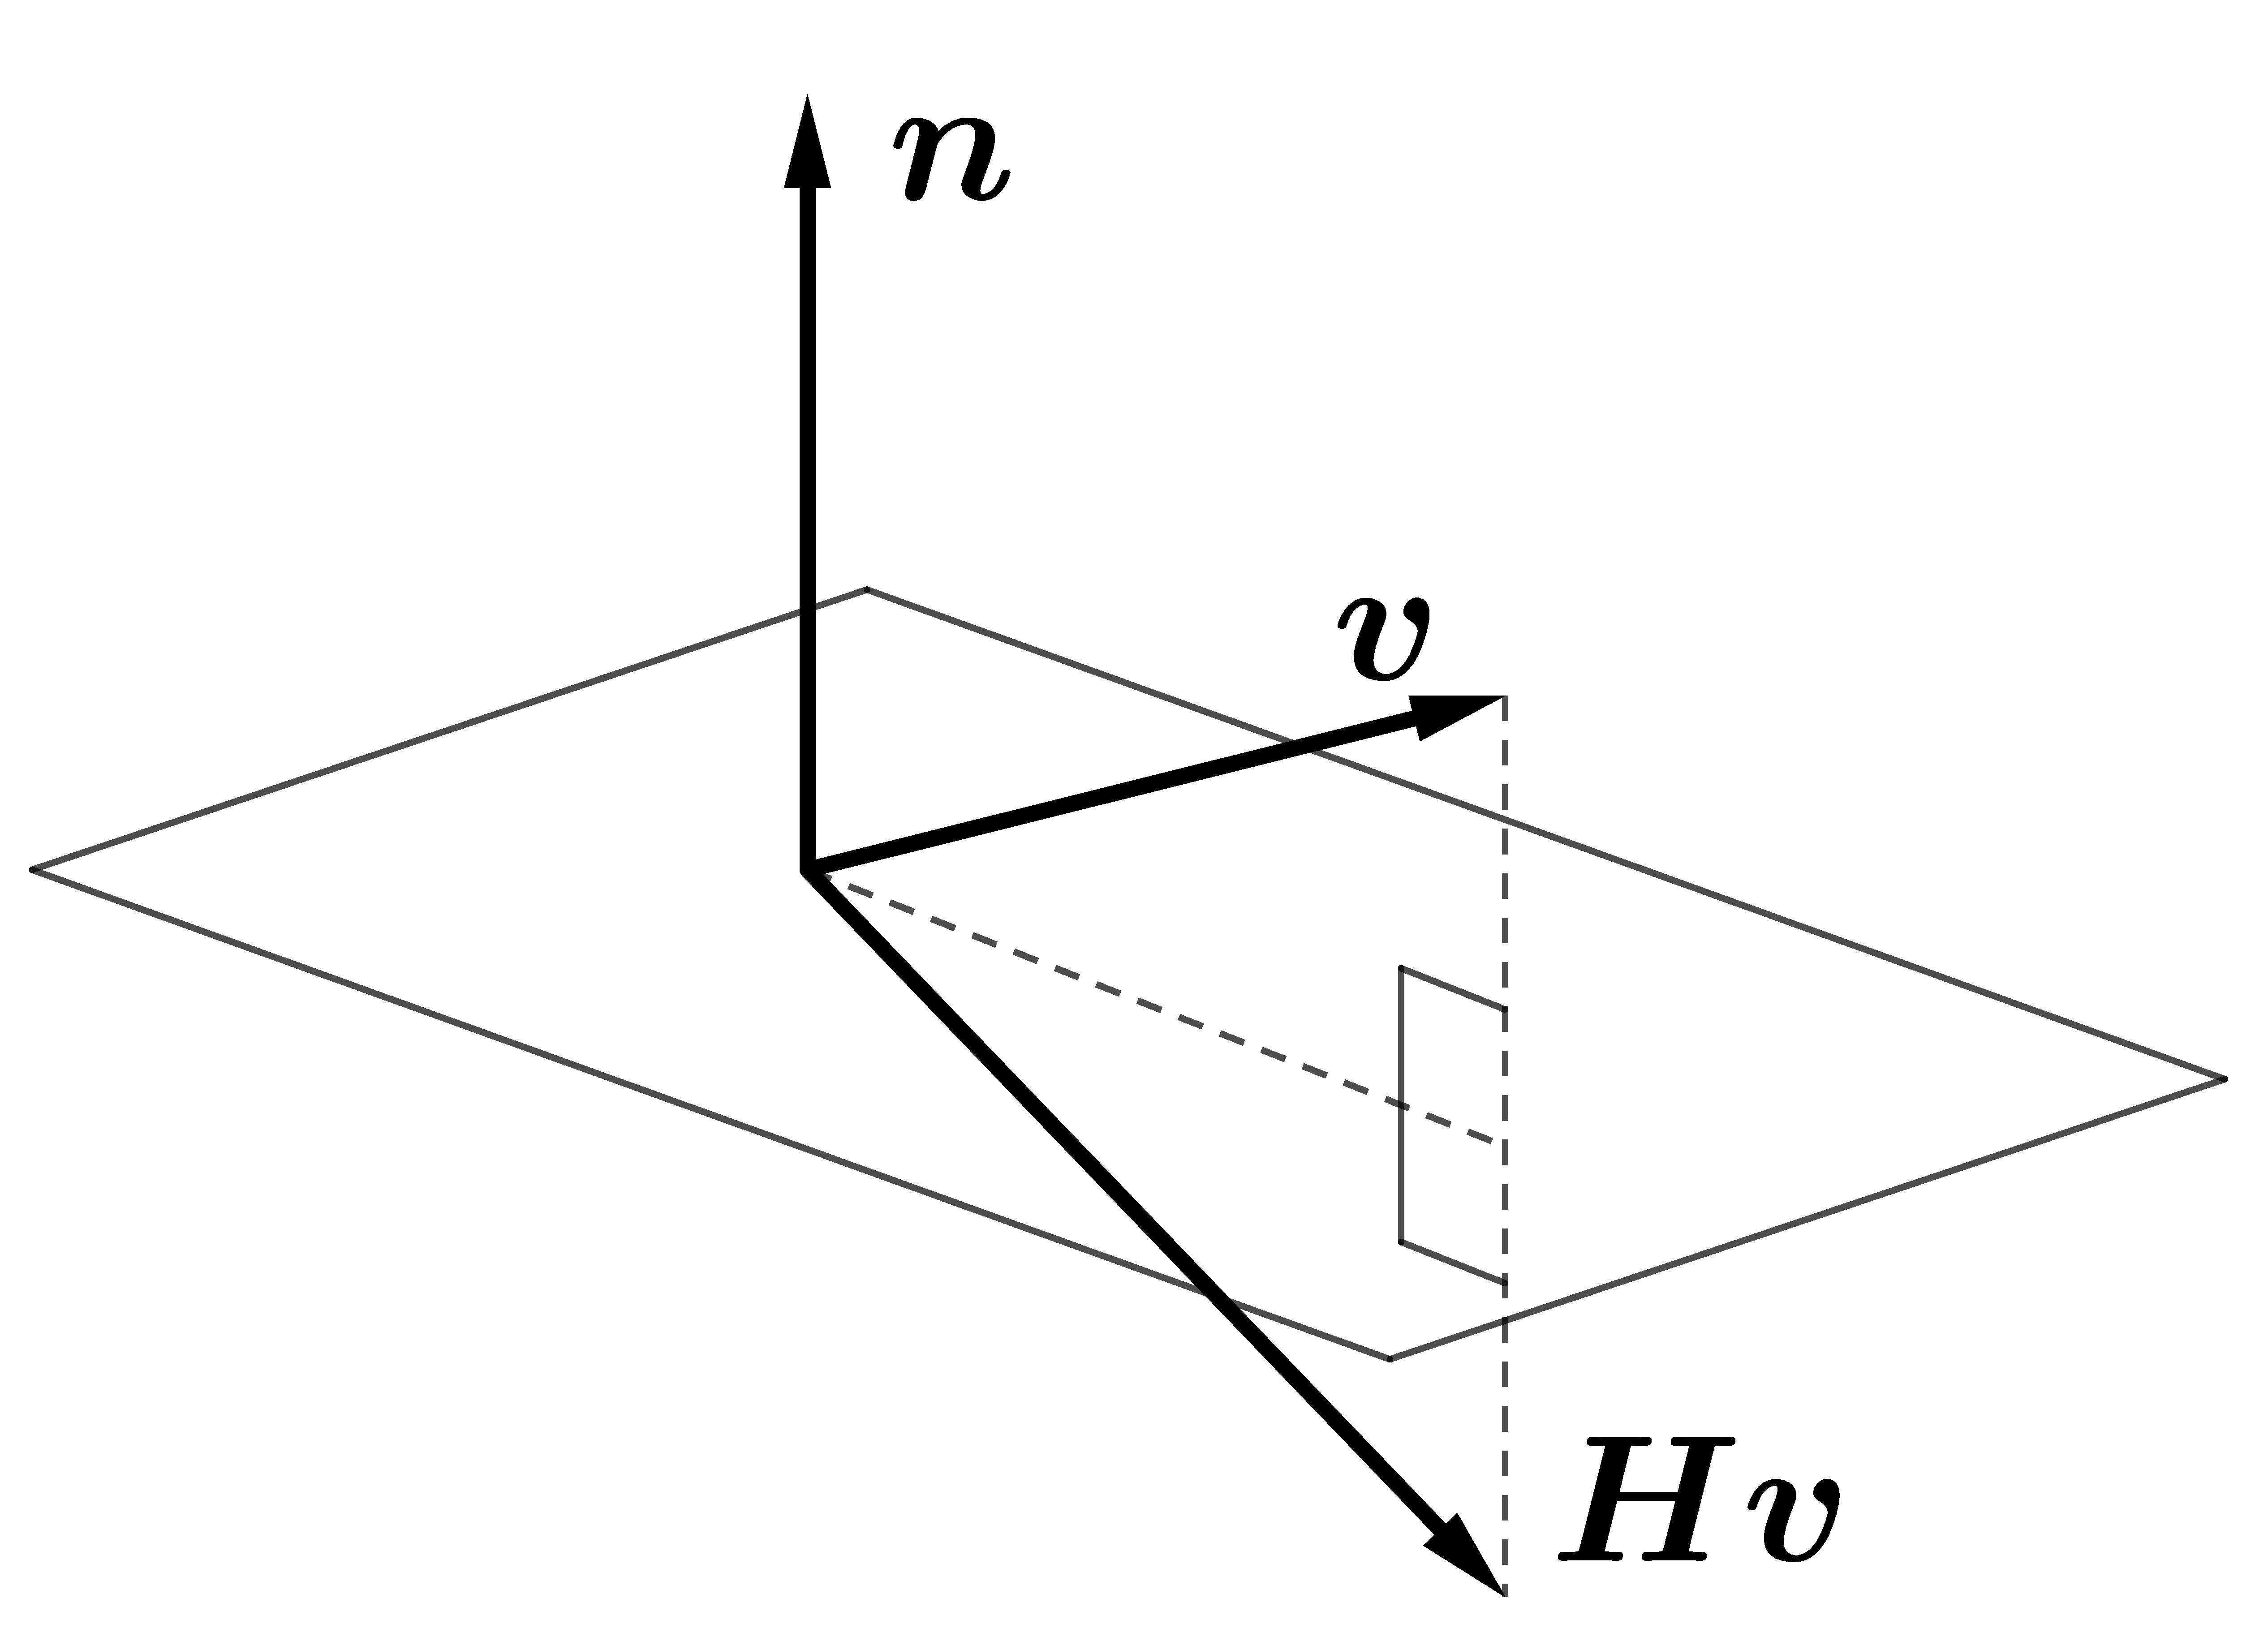
\includegraphics[width=0.85\textwidth]{./image/2.4.pdf}
            \caption{}
            \label{fig:2.4}
        \end{minipage}
        \begin{minipage}[b]{0.48\textwidth}
            \centering
            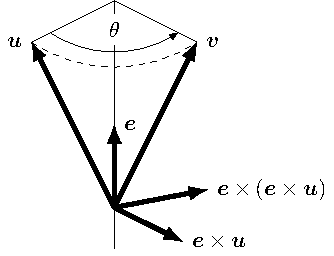
\includegraphics[width=0.85\textwidth]{./image/2.5.pdf}
            \caption{}
            \label{fig:2.5}
        \end{minipage}
    \end{figure}
    \item 三维旋转张量$\bb{R}$可以根据右手法则确定它的转轴、旋转方向$\bb{e}$和旋转角$\theta$。图\ref{fig:2.5}展示了矢量$\boldsymbol{v}=\boldsymbol{Ru}$的几何含义,即矢量$\bb{u}$围绕轴$\bb{e}$旋转角度$\theta $。
    \begin{enumerate}
        \item 将$\bb{v}$分解为三个彼此垂直的矢量$\boldsymbol{e},\boldsymbol{e}\times \boldsymbol{u},\boldsymbol{e}\times \left( \boldsymbol{e}\times \boldsymbol{u} \right) $的分量,证明:
        \begin{equation*}
            \begin{aligned}
                \boldsymbol{v}&=\boldsymbol{u}+\left( \sin \theta \right) \boldsymbol{e}\times \boldsymbol{u}+\left( 1-\cos \theta \right) \boldsymbol{e}\times \left( \boldsymbol{e}\times \boldsymbol{u} \right)\\
                &=\left( \cos \theta \right) \boldsymbol{u}+\left( 1-\cos \theta \right) \boldsymbol{e}\left( \boldsymbol{e}\cdot \boldsymbol{u} \right) +\left( \sin \theta \right) \boldsymbol{e}\times \boldsymbol{u}
            \end{aligned}
        \end{equation*}
        并因此有
        \begin{equation}\label{equ:2.41}
            \boldsymbol{R}=\left( \cos \theta \right) \mathbf{1}+\left( 1-\cos \theta \right) \boldsymbol{ee}+\left( \sin \theta \right) \boldsymbol{e}\times 
        \end{equation}
        \item 证明:$\bb{Re}=\bb{e}$
        \item 利用笛卡尔坐标,证明:$\det \bb{R}=+1$
        
        提示:设$\bb{e}_x=\bb{e}$
        \item 证明:
        \begin{equation*}
            \boldsymbol{R}^{\mathrm{T}}=\left( \cos \theta \right) \mathbf{1}+\left( 1-\cos \theta \right) \boldsymbol{ee}-\left( \sin \theta \right) \boldsymbol{e}\times 
        \end{equation*}
        \item 证明:对于有限旋转
        \begin{equation}\label{equ:2.42}
                \boldsymbol{r}=2\tan \left( \theta /2 \right) \boldsymbol{e}
        \end{equation}
        \begin{equation}
            \boldsymbol{R}=\left( 1+\frac{1}{4}\boldsymbol{r}\cdot \boldsymbol{r} \right) ^{-1}\left[ \left( 1-\frac{1}{4}\boldsymbol{r}\cdot \boldsymbol{r} \right) \mathbf{1}+\frac{1}{2}\boldsymbol{rr}+\boldsymbol{r}\times \right] \label{equ:2.43}
        \end{equation}
        (引入$\bb{r}$的优势在于式\eqref{equ:2.43}是关于$\bb{r}$分量的有理函数;不过,它在$\theta = \pi$处就变成了缺点。)
        \item 若$\boldsymbol{r}\sim \left( 1,1,1 \right) $,计算$\theta $和$\bb{R}$的笛卡尔坐标矩阵。
    \end{enumerate}
    \item 给定两个不平行的三维单位矢量,取$\sin \theta =\bb{u}\times \bb{v}$并利用式\eqref{equ:2.38}证明:旋转张量$\bb{R}$让$\bb{u}$绕垂直于$\bb{u}$和$\bb{v}$的转轴旋转得到矢量$\bb{v}$
    其定义为
    \begin{equation}\label{equ:2.44}
        \boldsymbol{R}=\mathbf{1}+\boldsymbol{vu}-\boldsymbol{uv}+\left( 1+\boldsymbol{u}\cdot \boldsymbol{v} \right) ^{-1}\left[ \left( \boldsymbol{uv}+\boldsymbol{vu} \right) \left( \boldsymbol{u}\cdot \boldsymbol{v} \right) -\left( \boldsymbol{uu}+\boldsymbol{vv} \right) \right] 
    \end{equation}
    由于\eqref{equ:2.44}不含叉积,因此它在任意维空间内均成立!(利用式\eqref{equ:2.39}和式\eqref{equ:2.40}或者式\eqref{equ:2.41}和式\eqref{equ:2.44},我们可以用两种不同的方式分别构造行列式等于$-1$或$+1$的正交张量。)
    \item 写出能将$\bb{e}_x$转换为$\boldsymbol{e}_x\cos \theta +\boldsymbol{e}_y\sin \theta $的旋转张量的$2\times 2$笛卡尔坐标矩阵。\
    \item 当$\boldsymbol{g}^i=\boldsymbol{g}_i$恒成立的时候,我们可以使用笛卡尔符号,也就是将所有的指标全部写成下标的形式。证明:当且仅当$\boldsymbol{g}_i=\boldsymbol{Qe}_i$时,我们才能这样操作,其中$\boldsymbol{Q}$是正交张量。通过引入笛卡尔标准基$\left\{ \boldsymbol{e}_i \right\} $和笛卡尔符号,我们很容易建立起相关等式。因此,借助式\eqref{equ:2.18}我们可以得到
    \begin{align*}
        \left( \boldsymbol{u}\times \boldsymbol{v} \right) \cdot \left( \boldsymbol{u}\times \boldsymbol{v} \right) &=\epsilon _{ijk}u_jv_k\epsilon _{iqr}u_qv_r\\
        &=\left( \delta _{jq}\delta _{kr}-\delta _{jr}\delta _{kq} \right) u_jv_ku_qv_r\\
        &=u_qv_ru_qv_r-u_rv_qu_qv_r\\
        &=\left( \boldsymbol{u}\cdot \boldsymbol{u} \right) \left( \boldsymbol{v}\cdot \boldsymbol{v} \right) -\left( \boldsymbol{u}\cdot \boldsymbol{v} \right) ^2
    \end{align*}
    \item 给定基底$\left\{ \boldsymbol{g}_1,\boldsymbol{g}_2,\boldsymbol{g}_3 \right\} $,请说明倒易基底$\left\{ \boldsymbol{g}^1,\boldsymbol{g}^2,\boldsymbol{g}^3 \right\} $的几何构型。
    \item 给定二维二阶张量$\boldsymbol{Tv}\sim \left( v_x,-v_y,v_x \right) $,其中$\boldsymbol{v}\sim \left( v_x,v_y \right) $
    \begin{enumerate}
        \item 写出它的对称部分$\bb{S}$和反对称部分$\bb{A}$
        \item 若$\bb{g}_1\sim (1,0),\bb{g}_2\sim (1,1)$,计算矩阵$\left[ T_{\cdot j}^{i} \right] ,\left[ T_{j}^{\cdot i} \right] ,\left[ S_{\cdot j}^{i} \right] $和$\left[ S_{j}^{\cdot i} \right] $。后两个矩阵对称吗?
    \end{enumerate}
    \item 设$\left\{ \boldsymbol{g}_i \right\} $是一个基底,$\bb{T}$为任意二阶张量,并令$\boldsymbol{h}_i=\boldsymbol{Tg}_i$
    \begin{enumerate}
        \item 证明:$\boldsymbol{T}=\boldsymbol{h}_i\boldsymbol{g}^i$
        \item 证明:$\frac{1}{2}\left( \boldsymbol{h}_i\boldsymbol{g}^i-\boldsymbol{g}^i\boldsymbol{h}_i \right) $是$\bb{T}$的反对称部分。
        \item 若$\bb{T}$是三维的,证明:$\frac{1}{2}\boldsymbol{g}^i\times \boldsymbol{h}_i$是反对称部分的转轴(见练习1.18)。
        \item 若$\left\{ \boldsymbol{g}_i \right\} $是由例题2.1给出的基底,并且$\boldsymbol{h}_1\sim \left( 1,0,-1 \right) ,\boldsymbol{h}_2\sim \left( 2,1,0 \right) ,\boldsymbol{h}_3\sim \left( 0,1,1 \right) $,计算$\bb{T}$的笛卡尔坐标和反对称部分的转轴。$\left\{ \boldsymbol{g}_i \right\} $由例题2.2的解答给出。
    \end{enumerate}
    \item 根据下面的思路,证明:由式\eqref{equ:2.41}定义的旋转张量$\bb{R}$可以写作指数形式
    \begin{equation}\label{equ:2.45}
        \boldsymbol{R}=\mathrm{e}^{\theta \boldsymbol{e}\times}=\mathbf{1}+\theta \boldsymbol{e}\times +\frac{\left( \theta \boldsymbol{e}\times \right) ^2}{2!}+\frac{\left( \theta \boldsymbol{e}\times \right) ^3}{3!}+\cdots 
    \end{equation}
    \begin{enumerate}
        \item 注意到
        \begin{equation}
            \boldsymbol{u}\times \boldsymbol{vw}=\left( \boldsymbol{u}\times \boldsymbol{v} \right) \boldsymbol{w}\,\, \text{以及} \,\, \boldsymbol{u}\times \mathbf{1}=\boldsymbol{u}\times 
        \end{equation}
        也即
        \begin{equation*}
            \left( \boldsymbol{u}\times \boldsymbol{vw} \right) \cdot \boldsymbol{x}=\left( \boldsymbol{u}\times \boldsymbol{v} \right) \boldsymbol{w}\cdot \boldsymbol{x}\,\, \text{以及} \,\, \left( \boldsymbol{u}\times \mathbf{1} \right) \cdot \boldsymbol{x}=\boldsymbol{u}\times \boldsymbol{x}\,\, \forall \boldsymbol{x}
        \end{equation*}
        证明:式\eqref{equ:1.49}表明
        \begin{equation*}
            \left( \boldsymbol{e}\times \right) ^2=\boldsymbol{ee}-1,\left( \boldsymbol{e}\times \right) ^3=-\boldsymbol{e}\times ,\left( \boldsymbol{e}\times \right) ^4=-\left( \boldsymbol{e}\times \right) ^2=-\left( \boldsymbol{ee}-1 \right) ,\cdots 
        \end{equation*}
        也即
        \begin{equation}\label{equ:2.25*}
            \left( \boldsymbol{e}\times \right) ^{2n}=\left( -1 \right) ^{n+1}\left( \boldsymbol{ee}-1 \right) \,\, , \,\, \left( \boldsymbol{e}\times \right) ^{2n+1}=\left( -1 \right) ^n\boldsymbol{e}\times \,\, ,\boldsymbol{n}=1,2,3,\cdots \tag{*}
        \end{equation}
        \item 在式\eqref{equ:2.42}中,我们置$\mathbf{1}\cos \theta =\mathbf{1}-\left( 1-\cos \theta \right) \mathbf{1}$,利用式\eqref{equ:2.25*}以及Taylor展开式
        \begin{equation*}
            \sin \theta =\theta -\frac{\theta ^3}{3!}+\cdots \,\, , \,\, 1-\cos \theta =\frac{\theta ^2}{2!}-\frac{\theta ^4}{4!}+\cdots 
        \end{equation*}
        来得到式\eqref{equ:2.45}。
    \end{enumerate}
    \item 若$\bb{e}$固定,$\bb{R}$仅为$\theta $的函数。找出一个$\bb{R}(\theta )$的带有初始条件的一阶微分方程。
    \item 正如任意一个非零复数$z$都可以表示为极坐标形式$z=r\mathrm{e}^{\mathrm{i}\theta},r>0$,每一个非奇异二阶张量$\bb{T}$都可以作极分解
    \begin{equation*}
        \boldsymbol{T}=\boldsymbol{V}\cdot \boldsymbol{R}=\boldsymbol{V}\cdot \mathrm{e}^{\theta \boldsymbol{e}\times}
    \end{equation*}
    其中,$\bb{V}$是正定对称张量,$\bb{R}$是旋转张量。给定$\bb{T}$,请运用你所学过的线性代数的知识分析如何先计算$\bb{V}$,然后再计算$\bb{R}$。
    \item 完成练习2.5,然后用相同的方法
    \begin{enumerate}
        \item 证明:若$A=\left[ A_{j}^{i} \right] $是一个$3\times 3$矩阵,那么式\eqref{equ:2.17}可以推广为
        \begin{equation}\label{equ:2.47}
            \epsilon^{i j k} \epsilon_{p q r} \operatorname{det} A=\left|\begin{array}{ccc}
                A_p^i & A_q^i & A_r^i \\
                A_p^j & A_q^j & A_r^j \\
                A_p^k & A_q^k & A_r^k
                \end{array}\right|
        \end{equation}
        \item 式\eqref{equ:2.18}的推广式是什么?
        \item 证明:通过取式\eqref{equ:2.47}中$q=j$以及$r=k$并将行列式按最右边一列展开,我们可以得到Cayley–Hamilton定理(“一个矩阵满足其自身的特征方程”):
        \begin{equation}
            A_j^i A_k^j A_p^k-\left(A_k^k\right) A_j^i A_p^j+\frac{1}{2}\left[\left(A_k^k\right)^2-A_k^j A_j^k\right] A_p^i-(\operatorname{det} A) \delta_p^i=0
        \end{equation}
        将之写作无指标形式,即为
        \begin{equation}
            A^3-(\operatorname{tr} A) A^2+\frac{1}{2}\left[(\operatorname{tr} A)^2-\operatorname{tr} A^2\right] A-(\operatorname{det} A) I=0
        \end{equation}

    \end{enumerate}
\end{exercise}
